\documentclass[12pt]{article}
\usepackage[pdftex]{graphicx}
\usepackage{%
	amsfonts,%
	amsmath,%	
	amssymb,%
	amsthm,%
%	babel,%
	bbm,%
	%biblatex,%
	caption,%
	centernot,%
	color,%
	enumerate,%
	epsfig,%
	epstopdf,%
	etex,%
	geometry,%
	graphicx,%
	hyperref,%
	latexsym,%
	mathtools,%
	multicol,%
	pgf,%
	pgfplots,%
	pgfplotstable,%
	pgfpages,%
	proof,%
	psfrag,%
	subfigure,%	
	tikz,%
	ulem,%
	url%
}	

\usepackage[mathscr]{eucal}
\usepgflibrary{shapes}
\usetikzlibrary{%
  arrows,%
  backgrounds,%
  chains,%
  decorations.pathmorphing,% /pgf/decoration/random steps | erste Graphik
  decorations.text,%
  matrix,%
  positioning,% wg. " of "
  fit,%
  patterns,%
  petri,%
  plotmarks,%
  scopes,%
  shadows,%
  shapes.misc,% wg. rounded rectangle
  shapes.arrows,%
  shapes.callouts,%
  shapes%
}

\theoremstyle{plain}
\newtheorem{thm}{Theorem}[section]
\newtheorem{lem}[thm]{Lemma}
\newtheorem{prop}[thm]{Proposition}
\newtheorem{cor}[thm]{Corollary}

\theoremstyle{definition}
\newtheorem{defn}[thm]{Definition}
\newtheorem{conj}[thm]{Conjecture}
\newtheorem{exmp}[thm]{Example}
\newtheorem{assum}[thm]{Assumptions}
\newtheorem{axiom}[thm]{Axiom}

\theoremstyle{remark}
\newtheorem{rem}[thm]{Remark}
\newtheorem{note}[thm]{Note}

\newcommand{\norm}[1]{\left\lVert#1\right\rVert}
\newcommand{\indep}{\!\perp\!\!\!\perp}
\DeclarePairedDelimiter\abs{\lvert}{\rvert}%
%\DeclarePairedDelimiter\norm{\lVert}{\rVert}%
\newcommand{\tr}{\operatorname{tr}}
\newcommand{\R}{\mathbb{R}}
\newcommand{\Q}{\mathbb{Q}}
\newcommand{\N}{\mathbb{N}}
\newcommand{\E}{\mathbb{E}}
\newcommand{\Z}{\mathbb{Z}}
\newcommand{\B}{\mathscr{B}}
\newcommand{\C}{\mathcal{C}}
\newcommand{\T}{\mathscr{T}}
\newcommand{\F}{\mathcal{F}}
\newcommand{\G}{\mathcal{G}}
%\newcommand{\ba}{\begin{align*}}
%\newcommand{\ea}{\end{align*}}

% Debug
\newcommand{\todo}[1]{\begin{color}{blue}{{\bf~[TODO:~#1]}}\end{color}}


\makeatletter
\def\th@plain{%
  \thm@notefont{}% same as heading font
  \itshape % body font
}
\def\th@definition{%
  \thm@notefont{}% same as heading font
  \normalfont % body font
}
\makeatother
\date{}
\usepackage{tabu}

\begin{Huge}
	\title{SPQT PROJECT REPORT \\CHARACTERIZATION OF ECONOMY}
\end{Huge}

\begin{document}
\maketitle


\begin{large}
\begin{center}
	Manju M Raj\\
	Nanditha Unnikrishnan\\
\end{center}	
\end{large}



\newpage
\tableofcontents

\newpage

\section{INTRODUCTION}

On November 8$^{th}$,Indian government took a historic decision by announcing that the high-denomination notes (Rs. 500 and Rs. 1,000) then in circulation would cease to be legal tender.
With demonetization effort 86 percentage of Indian currency was nullified that aimed to wash the stock of ‘black market's cash supply’ and counterfeit notes out of the economy and convert it into the licit, banked and taxable, part of the economy.
The move has led to a shortage of lower denomination notes such as Rs 100 and Rs 50 that are still legal tender, as people have taken to conserving whatever cash they have in hand. The demonetization initiative has caused a sudden breakdown in India’s commerce and the unbanked and informal economy was hard hit. Trade across all aspects of the economy has interrupted, and sectors like agriculture, fishing, and the huge informal market were almost shut down during the initial days of announcement. The informal sector in India employs more than a majority of the workers and most transactions are in cash.
\\
Since our economy is heavily dependent on cash, as only less than half the population uses banking system for monetary transactions, demonetization hit trade and consumption hard. With people scrambling for cash to pay for goods and services, the move took a big toll on the country's growth and output during the then fiscal. 


\section{PROBLEM STATEMENT}
Our aim is to characterize the effects of demonetization on consumption. We want to predict out how much time it takes for the economy to stabilize after the disturbance caused by demonetization. \\
Majority of Indian population depends on cash-in-hand rather than banking system for consumption.
Therefore it is sufficient to model cash-in-hand as a stochastic process to study the effects.


\section{LITERATURE SURVEY}
\begin{itemize}
  \item \textit{Stochastic Implications of the Life Cycle-Permanent Income Hypothesis: Theory and Evidence (Robert E Hall)}\\
  The paper is based on the life cycle – permanent income hypothesis and models consumption as a random walk process. The paper suggests that no other information apart from the consumption at time 't' helps to predict the future consumption. The income or wealth in periods 't' or earlier are irrelevant.
  \paragraph{}
  For policy analysis, the pure life cycle permanent hypothesis supports the view that unexpected changes in policy, affect consumption only to the extent that they affect permanent income. But in the case of demonetization, the permanent income is not affected and hence, modeling consumption as random walk in the scenario with demonetization would provide false results.\\With the literature survey conducted by us, we were not able to find any paper which takes into     consideration the cash-in-hand (the only quantity directly affected by demonetization). Therefore we developed a new model of cash-in-hand as a Discrete Time Markov Process.
  \item To implement the model, data were collected from the website of Reserve Bank of India. Monetary policies regarding the limit on withdrawals from ATM during the months November 2016 –February 2017 were observed.
  \begin{table}[h]
\centering
\caption{Changes in Monetary Policy}
\begin{tabu} to 0.8\textwidth { | X[l] | X[c] | X[c] | X[c] | }
 \hline
  Date & Daily limit (in Rs.) & Limit of withdrawal from bank & Weekly limit (in Rs.) \\
 \hline
 10$^{th}$ Nov'16 & 2000 & 10000 & 20000 \\
 \hline
 18$^{th}$ Nov'16& 2500 & 10000 & 24000 \\
\hline 
  1$^{st}$ Jan'17& 4500  & 10000 & 24000 \\
\hline
 
 17$^{th}$ Jan'17 & 10000  & 10000 & 24000 \\
 \hline
 20$^{th}$ Feb'17& 10000  & 10000 & 50000 \\
 \hline
 13$^{th}$ Mar'17& 10000  & 10000 & No limit \\
 \hline
\end{tabu}
\end{table}

\item Mixing Time: \\
The mixing time of a Markov chain is defined as the time taken for the Markov chain to attain its stationary distribution.
\\\\Let P$_{i,j}$ denote the transition probability from state i to j and $\pi^{T}$ = [ $\pi_{1}$ $\pi_{2}$ $\cdots$ $\pi_{M}$ ] denote the stationary distribution of the markov chain.\\In [1], the time to mixing is defined as follows.
\\Let Y be a random variable with probability mass function given by $\pi^{T}$. A  markov chain ${X_{n}}$ is said to achieve
“mixing”, at time T = k, when $X_{k}$ = Y for the smallest such k $\geq$ 1.Sample a value from $\lbrace$ $\pi_{j}$ $\rbrace$ to get a value for Y, say Y = j.Observe the markov chain starting from any state, say i . 
\begin{center}
$T_{ij}$ = min$\lbrace$ n $\geq$ 1 such that $X_{n}$ = j given that $X_{0}$ = i$\rbrace$  
\end{center}
Then expected time to mixing starting from a state i, $\eta_{i}$ is given by,
\begin{center}
$m_{ij}$ = E [  $T_{ij}$ $|$ $X_{0}$ = i ]\\
$\eta_{i}$  = $\Sigma^{m}_{j=1}$ $m_{ij}$ $\pi_{j}$
\end{center}

From the Transition Probability Matrix ,P $\eta$s can be calculated as follows:\\
Let $e^{T}$ = [ 1 1 1 $\cdots$ 1]$_{(1 \times M)}$

E = e$e^{T}$ = [1]$_{(M \times M)}$, \hspace{2pt}      M=[$m_{ij}$],

M$_{d}$=[$\delta_{ij}$m$_{ij}$], \hspace{2pt}
$\Pi$ = e$\pi^{T}$ \\
Let G := g-inverse of (I-P) \\
Generalized inverse (g-inverse) of a matrix A is D if ADA = A. \\
H = G( I - $\Pi$),\hspace{2pt}, C = I - H ,\hspace{2pt} C$_{d}$=[$\delta_{ij}$C$_{ij}$]
\begin{equation}
M = [ C - EC_{d} + E ]D\\
\eta_{i} = M_{i} \pi^{T}
\end{equation}
where $M_{i}$ is the $i^{th}$ row of matrix M.
In [2] ,it has been proved that $\eta_{i}$s are independent of i.\\
An alternate way to calculate mixing times has also been presented in [1].
For an irreducible Markov chain $\lbrace$X$_{n}\rbrace$, and p$_{j}$(n) = 
P$\lbrace$X$_{n}$ = j$\rbrace$ and
stationary distribution $\lbrace\pi_{j}\rbrace$, define the entropy
\begin{center}
E(n)= -$\Sigma_{j}$ p$_{j}$(n)log $\frac{p_{j}(n)}{\pi_{j}}$
\end{center}
For m $\geq$ 1, E(n + m) $\geq$ E(n), with equality if and only if p$_{j}$(n) = $\pi_{j}$ for all
j. Hence the “mixing time” is just the minimal integer such that the equality holds. This justifies
the view that the “mixing time” is really the “time to stationarity”.
\end{itemize}

\section{SYSTEM MODEL}
The cash-in-hand is modeled as a Discrete Time Markov Process. The state space of this DTMC consists of the discretized versions of cash-in-hand as multiples of 500s truncated at Rs.10,000.
\begin{center}
\textit{E} = $\lbrace$ 500 $*$ n, n=0,1,2,3,$\cdots$ 20$\rbrace$
\end{center}
The transitions among these state spaces are caused by inflow of cash (mostly by ATM withdrawals) and consumption. The Transition Probability Matrix of this DTMC is a 21x21 matrix. The inter-arrival times between each withdrawals and consumption events are assumed to be geometrically distributed.\\
We have considered two separate scenarios: before and after demonetization (Nov 8th). \\
Assume that the DTMC already follows stationary distribution before demonetization. 
On November 8th, demonetization acted as a disturbance to this DTMC which had achieved stationarity, thereby changing the Transition Probability Matrix (TPM) to a great extent. \\We made observations in the time period of four months from November 2016 to February 2017, during which the economic policies deciding the limit of withdrawal from banks kept changing. With any change in the policy, the TPM also changes. By February, the withdrawal limits were restored to the values before demonetization.  We have assumed that after January 17th the TPM became almost same as the one before demonetization was put in effect, the DTMC may not have achieved stationary distribution though.\\ With the same TPM and a different distribution, the mixing times can be calculated. The expected value of mixing time will provide an estimate of the time for the economy to stabilize.

\section{WORK DONE}
In this project we are considering only the middle class population. We collected bank statements of 100 people from October 2016 to February 2017.\\ As curve-fitting to an already existing probability distribution could not be done to the data collected, we empirically calculated the probability of withdrawals and consumption of each value in state space.\\For example, probability of withdrawing Rs.500 = (Number of times Rs.500 was withdrawn from ATMs)/(Total number of withdrawals from ATMs).\\For a 31-day month, total number of withdrawals by 100 people = 31 x 100 ,assuming 'Rs.0' withdrawals are also possible.
 \begin{table}[h]
\centering
\caption{Withdrawal Data(As number of withdrawals)}

\begin{tabu} to 0.8\textwidth { | X[l] | X[c]  | X[c] | X[c] | X[c] | }
 \hline
 
  Amount Withdrawn  & Oct-Nov & Nov-Dc & Dec-Jan & Jan-Feb \\
 \hline
 0 & 2524 & 2707 & 2706 & 2612 \\
 \hline
 500 & 110 & 80 & 106 & 106 \\
 \hline
 1000 & 80 & 27 & 49 & 68 \\
 \hline
 1500 & 55 & 16 & 35 & 42 \\
 \hline
 2000 & 67 & 93 & 102 & 127 \\
 \hline
 2500 & 15 & 37 & 14 & 42 \\
 \hline
 3000 & 28 & 5 & 8 & 13\\
 \hline
 3500 & 4 & 1 & 12 & 18 \\
 \hline
 4000 & 17 & 5 & 25 & 14 \\
 \hline
 4500 & 20 & 8 & 10 & 22 \\
 \hline
 5000 & 40 & 6 & 15 & 7 \\
 \hline
 5500 & 22 & 1 & 1 & 1 \\
 \hline
 6000 & 17 & 1 & 2 & 8 \\
 \hline
 6500 & 14 & 1 & 1 & 2 \\
 \hline
 7000 & 25 & 2 & 1 & 1 \\
 \hline
 7500 & 19 & 4 & 1 & 1 \\
 \hline
 8000 & 11 & 1 & 2 & 4 \\
 \hline
8500 & 9 & 1 & 1 & 1\\
 \hline
9000 & 2 & 1 & 1 & 2 \\
 \hline
 9500 & 1 & 1 & 1 & 1\\
 \hline
 10000 & 20 & 2 & 7 & 8 \\
 
 \hline
\end{tabu}
\end{table}

 \begin{table}[h]
\centering
\caption{Consumption Data(As number of spendings)}

\begin{tabu} to 0.8\textwidth { | X[l] | X[c]  | X[c] | X[c] | X[c] | }
 \hline
 
Expenditure per day (in Rs.)  & Oct-Nov & Nov-Dc & Dec-Jan & Jan-Feb \\
 \hline
 0 & 415 & 1141 & 1097 & 621 \\
 \hline
 500 & 1919 & 1472 & 1435 & 1811 \\
 \hline
 1000 & 424 & 205 & 379 & 390 \\
 \hline
 1500 & 142 & 47 & 51 & 114 \\
 \hline
 2000 & 70 & 43 & 40 & 54 \\
 \hline
 2500 & 46 & 20 & 17 & 30 \\
 \hline
 3000 & 10 & 12 & 14 & 8\\
 \hline
 3500 & 13 & 8 & 9 & 6 \\
 \hline
 4000 & 17 & 11 & 16 & 12 \\
 \hline
 4500 & 7 & 6 & 4 & 8 \\
 \hline
 5000 & 19 & 12 & 18 & 14 \\
 \hline
 5500 & 2 & 3 & 1 & 7 \\
 \hline
 6000 & 3 & 1 & 2 & 11 \\
 \hline
 6500 & 4 & 2 & 1 & 2 \\
 \hline
 7000 & 1 & 2 & 1 & 1 \\
 \hline
 7500 & 1 & 2 & 2 & 3 \\
 \hline
 8000 & 2 & 4 & 3 & 3 \\
 \hline
8500 & 1 & 1 & 3 & 1\\
 \hline
9000 & 1 & 3 & 2 & 1 \\
 \hline
 9500 & 1 & 1 & 4 & 1\\
 \hline
 10000 & 2 & 4 & 1 & 2 \\
 
 \hline
\end{tabu}
\end{table}



\subsection{TPM Construction}
Let $\lbrace$P$_{k}$,k$\geq$0$\rbrace$ denote the DTMC under consideration.\\
$\lbrace$A$_{k}$,k$\geq$0$\rbrace$ : Withdrawal process\\ 
$\lbrace$C$_{k}$,k$\geq$0$\rbrace$ : Consumption process\\ 
\begin{center}
P$_{k+1}$ = P$_{k}$ + A$_{k}$ - C$_{k}$\\


\end{center}

\begin{eqnarray}
Pr(P_{k+1} = j | P_{k} = i)&=&Pr(P_{k} + A_{k} - C_{k} = j | P_{k} = i) \\
&=&Pr(  i + A_{k} - C_{k} = j | P_{k}  = i)\\
&=&Pr(  A_{k} - C_{k} = j-i )\\
&=&\mathbb{E} [ 1_{\lbrace A_{k} - C_{k} = j-i \rbrace} ] \\
&=&\mathbb{E}[\mathbb{E} [ 1_{\lbrace A_{k} - C_{k} = j-i \rbrace}|C_{k} = c ] ]\\
&=&\mathbb{E}[\mathbb{E}[1_{\lbrace A_{k} = j-i+c \rbrace}|C_{k} = c ]] \\
&=&\sum_{x\in\textit{E}} Pr(A_{k} = j-i+c).Pr(C_{k} = c)
\end{eqnarray}

The transition probability from state i to j is given by
\begin{equation}
p_{ij} = \frac{Pr(P_{k+1} = j | P_{k} = i)}{\sum_{j\in\textit{E}}Pr(P_{k+1} = j | P_{k} = i)}
\end{equation}

\paragraph{}
The inter-arrival times of withdrawal and consumption processes are geometrically distributed with parameters given by
\begin{center}
 pwithdrawal = 1 - Pr(zero withdrawal)\\
 pconsumption = 1 - Pr(zero consumption)
\end{center}
\subsection{Two cases}
We considered two cases towards end of February(When the financial policy was restored as before):\\
\begin{itemize}
	\item TPM same as that before demonetization 
	\item TPM with small perturbations \\
	$\overline{P}$=P+$\textbf{E}$, \hspace{2pt} where $\textbf{E}$=[$\epsilon_{ij}$] is the matrix of perturbations with the property that $\sum_{j=1}^{M}\epsilon_{ij}$=0\\
	Let $\pi^{T}$ and $\overline{\pi}^{T}$ be the stationary probability vectors for P and $\overline{P}$ respectively.\\
	From [3], it can be shown that for an irreducible M state Markov chin undergoing a general perturbation $\textbf{E}$=[$\epsilon_{ij}$]\\
	\begin{equation}
		\| \pi - \overline{\pi}\|_{1} \leq (\eta-1)\|\textbf{E}\|_{\infty}
	\end{equation}
\end{itemize}


\section{RESULTS}

Expected Mixing time :From the end of February 2017
\begin{itemize}
\item From Eqn (1) : 21 days (Without perturbation)
\item From MATLAB simulations : 24 days (Without perturbation)
\item From Eqn(10) : 28 days (With perturbation)
\end{itemize}

Probability distribution curves of withdrawal and consumption values are plotted below\\ \\ \\ \\ \\ \\ \\


\begin{figure}
	\centering
	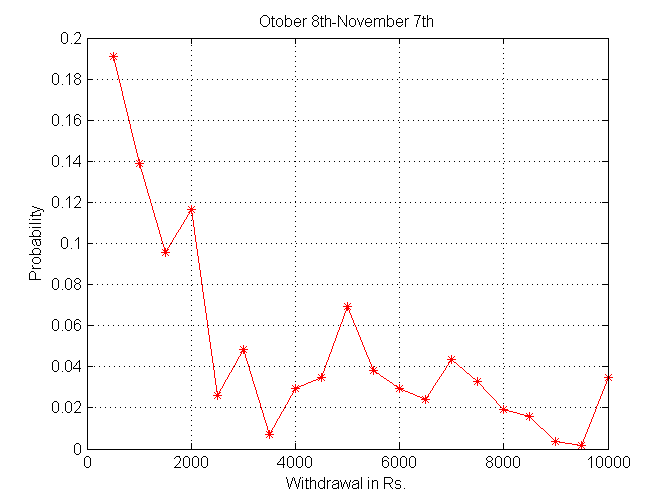
\includegraphics[scale=0.65]{WOCT.png}
	\caption{}
	\label{fig:fig1}
\end{figure}
\begin{figure}
	\centering
	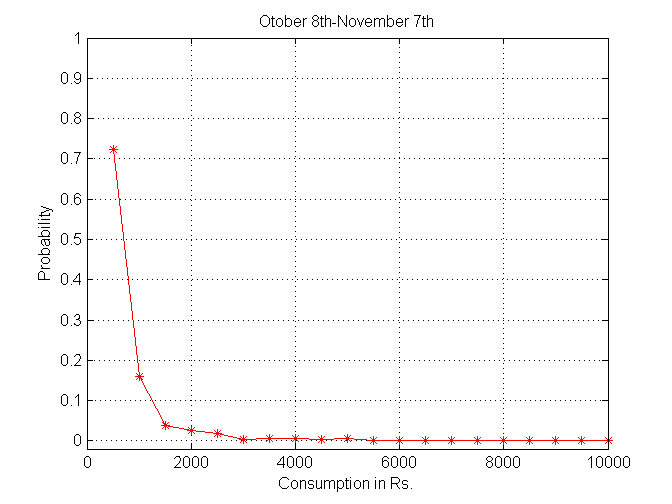
\includegraphics[scale=0.65]{COCT.png}
	\caption{}
	\label{fig:fig2}
\end{figure}

\begin{figure}
	\centering
	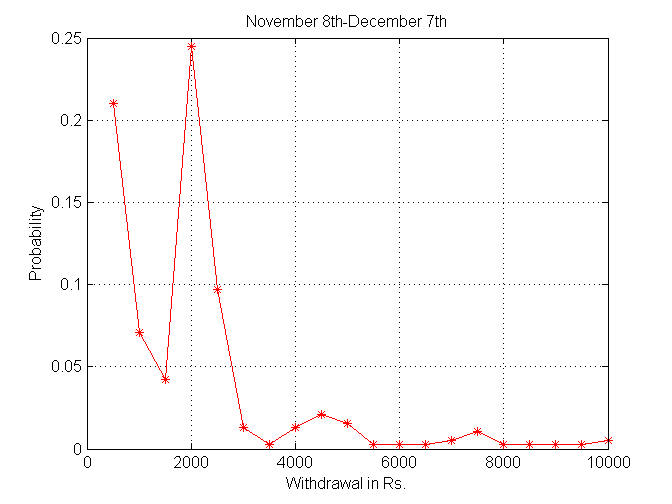
\includegraphics[scale=0.65]{WNOV.png}
	\caption{}
	\label{fig:fig3}
\end{figure}
\begin{figure}
	\centering
	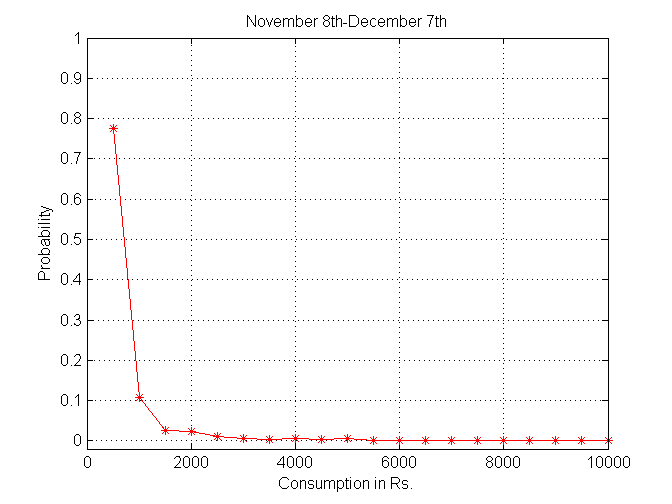
\includegraphics[scale=0.65]{CNOV.png}
	\caption{}
	\label{fig:fig4}
\end{figure}
\begin{figure}
	\centering
	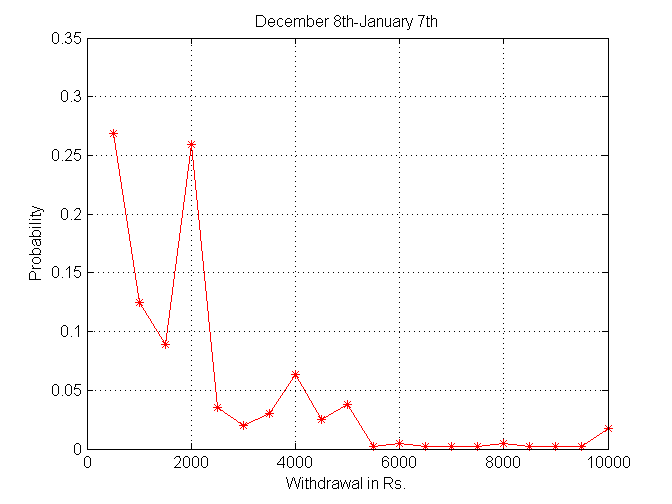
\includegraphics[scale=0.65]{WDEC.png}
	\caption{}
	\label{fig:fig5}
\end{figure}
\begin{figure}
	\centering
	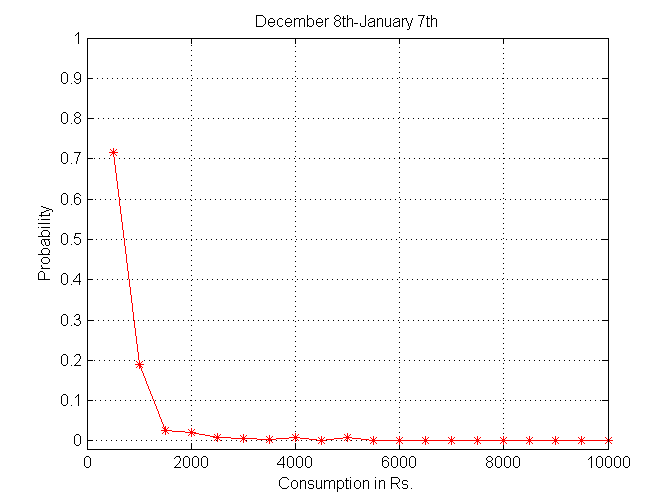
\includegraphics[scale=0.65]{CDEC.png}
	\caption{}
	\label{fig:fig6}
\end{figure}
\begin{figure}
	\centering
	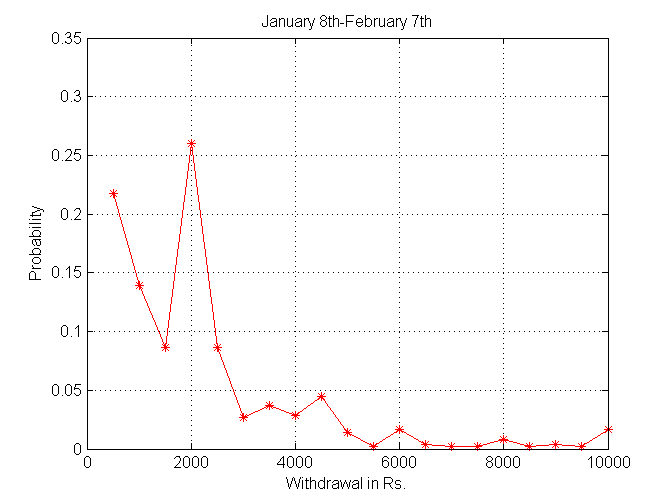
\includegraphics[scale=0.65]{WJAN.png}
	\caption{}
	\label{fig:fig7}
\end{figure}
\begin{figure}
	\centering
	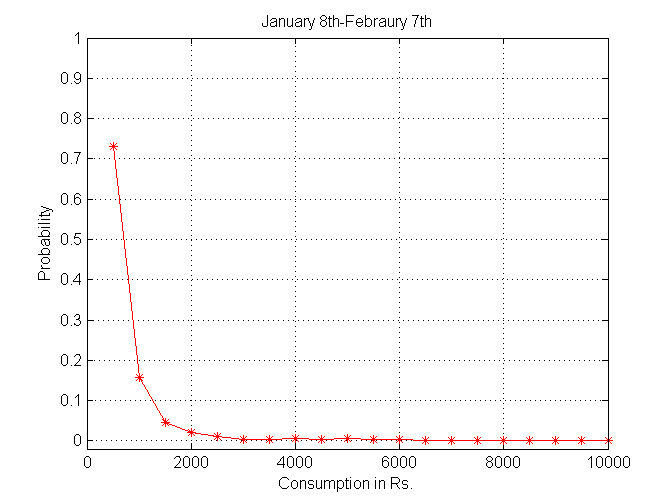
\includegraphics[scale=0.65]{CJAN.png}
	\caption{}
	\label{fig:fig8}
\end{figure}


\newpage
\section{REFERENCE}
\begin{scriptsize}

\begin{small}
$[1]$ Jeffrey J. Hunter, "Coupling and Mixing times in Markov chains", Res.Lett.Inf. Math.Sci.(2007) 11, 1-22.\\
$[2]$ Hunter J.J., "Mixing times with applications to perturbed Markov chains", Linear Algebra Appl.,417, 108-123 (2006). \\
$[3]$ Hunter J.J., "Stationary distributions and mean first passage times of perturbed Markov chains, Linear Algebra Appl., 410 (2005) 217-243. \\
$[4]$ Robert E. Hall, "Stochastic implications of the life cycle-permanent income hypothesis:theory and evidence", Journal of Political Economy, 1978, Vol.86, No.6.
 \\
$[5]$ https://www.rbi.org.in/Scripts/NotificationUser.aspx\\
\end{small}
\end{scriptsize}




 







\end{document}
